\documentclass[sigconf,nonacm]{acmart}

%% Strip ACM boilerplate
\setcopyright{none}
\settopmatter{printacmref=false}
\renewcommand\footnotetextcopyrightpermission[1]{}
\pagestyle{plain}

%% ── Packages ──────────────────────────────────────────────────────────────
\usepackage{booktabs}
\usepackage{tabularx}
\usepackage{adjustbox}
\usepackage{multirow}
\usepackage{makecell}      % \thead, line breaks in cells
\usepackage{array}
\usepackage{microtype}
\usepackage{url}
\urlstyle{rm}
\usepackage{enumitem}
\usepackage{listings}
\usepackage{xcolor}
\usepackage{tikz}
\usetikzlibrary{shapes.geometric, arrows.meta, positioning,
                fit, backgrounds, calc, matrix}

%% ── Colours ───────────────────────────────────────────────────────────────
\definecolor{phase1}{HTML}{1A5276}
\definecolor{phase2}{HTML}{117A65}
\definecolor{phase3}{HTML}{6E2F8A}
\definecolor{idcol}  {HTML}{2C3E50}
\definecolor{devcol} {HTML}{1A5276}
\definecolor{netcol} {HTML}{117A65}
\definecolor{appcol} {HTML}{922B21}
\definecolor{attackred}{HTML}{C0392B}
\definecolor{supplyorg}{HTML}{E67E22}
\definecolor{lightbg} {HTML}{F4F6F7}
\definecolor{midgray}  {HTML}{BDC3C7}
\definecolor{codebg}   {HTML}{F2F3F4}

%% ── Listings style (for DID document) ────────────────────────────────────
\lstset{
  backgroundcolor=\color{codebg},
  basicstyle=\ttfamily\fontsize{6.2pt}{7.5pt}\selectfont,
  breaklines=true,
  frame=single,
  rulecolor=\color{midgray},
  columns=flexible,
  keepspaces=true,
  showstringspaces=false,
  numbers=none,
  xleftmargin=4pt, xrightmargin=4pt,
  aboveskip=4pt, belowskip=4pt,
}

%% ── Metadata ──────────────────────────────────────────────────────────────
\title{Post-Quantum Cryptography, Decentralised Identity, and Modern
Zero Trust IAM: Standards, Compliance, Attacker Adaptation, and
Resilience}

\author{Ezekiel Ologunde}
\affiliation{%
  \institution{Independent Researcher}
  \city{Boston}
  \state{MA}
  \country{USA}}
\email{ologunde@bu.edu}

\begin{document}

\begin{abstract}
The convergence of post-quantum cryptography (PQC) and decentralised
identity (DID) is redefining the cryptographic foundations of Zero
Trust Architecture (ZTA).  NIST's 2024 finalisation of FIPS~203
(ML-KEM), FIPS~204 (ML-DSA), and FIPS~205 (SLH-DSA) provides the
first production-ready PQC suite; W3C DIDs and the emerging Multikey
and JOSE-PQC specifications supply the identity-layer migration
pathway.  Simultaneously, modern IAM platforms are displacing
passwords with FIDO2/WebAuthn passkeys, just-in-time (JIT) privilege,
and continuous access evaluation, while global regulators---OMB
M-22-09, DoD ZT Strategy, NYDFS Part~500, and DORA---mandate ZTA
controls at statutory deadlines.

This paper makes six contributions: (1)~a technical analysis of
PQC-DID integration covering hybrid DID documents, IETF JOSE/COSE
drafts, and a phased migration strategy; (2)~a comparative survey of
eight IAM vendors; (3)~a compliance-to-ZTA-control mapping for six
regulatory frameworks; (4)~an attacker-adaptation analysis with five
evolved threat profiles and mitigations; (5)~UX best practices grounded
in operational data; and (6)~a resilience architecture addressing ZTA
graceful degradation during identity-system outages.
\end{abstract}

\keywords{Post-Quantum Cryptography; Decentralized Identity; DID;
ML-KEM; ML-DSA; FIDO2; IAM; Zero Trust; JIT Access; NYDFS;
OMB~M-22-09; Resilience; Hybrid Cryptography}

\maketitle

\paragraph{Methodological Disclosure.} The IAM vendor pricing figures in this paper (e.g., approximately \$3k/month and \$9/user/month) are drawn from vendor pricing pages at the time of writing, are indicative rather than verified, and may have changed since. The statement that a mature Zero Trust Architecture still blocks only approximately half of attacks is drawn from a single Dark Reading article and has not been independently corroborated; both figures should be treated as unverified, time-sensitive secondary-source claims.

%% ═══════════════════════════════════════════════════════════════════════════
\section{Introduction}
%% ═══════════════════════════════════════════════════════════════════════════

Two converging forces are reshaping ZTA foundations.  The
\emph{quantum threat}---sufficiently powerful quantum computers will
break RSA, ECDH, and ECDSA---undermines every current DID, TLS
handshake, and access token.  The \emph{identity-centric security
imperative}---credential compromise now dominates attack
vectors---drives regulators to mandate phishing-resistant MFA,
continuous verification, and least-privilege at statutory deadlines.

NIST finalised its first three PQC standards in August 2024, providing
the first production-ready post-quantum algorithm suite~\cite{nist204}.
The ``harvest now, decrypt later'' attack---capturing today's encrypted
DID traffic for future quantum decryption---makes immediate hybrid
deployment urgent even before quantum computers are practically
available~\cite{linkedin2024}.

\subsection*{Paper Contributions}
\begin{enumerate}[leftmargin=*, label=(\arabic*), topsep=2pt, itemsep=1pt]
  \item PQC-DID technical analysis: hybrid documents, IETF drafts, migration phases.
  \item IAM vendor comparison across eight platforms.
  \item Compliance mapping of six regulatory frameworks to ZTA controls.
  \item Attacker adaptation: five evolved TTPs with structured mitigations.
  \item UX best practices with operational metrics.
  \item Resilience architecture for graceful degradation.
\end{enumerate}

%% ═══════════════════════════════════════════════════════════════════════════
\section{Post-Quantum Cryptography and Decentralised Identity}
%% ═══════════════════════════════════════════════════════════════════════════

\subsection{NIST PQC Algorithm Suite}

NIST's 2024 finalisations~\cite{nist204,ping2024federal} establish
three standards:

\textbf{FIPS~203 -- ML-KEM (Kyber).}  Module-Lattice Key Encapsulation
Mechanism.  Replaces ECDH/RSA-OAEP for key exchange.

\textbf{FIPS~204 -- ML-DSA (Dilithium).}  Module-Lattice Digital
Signature Algorithm.  Replaces ECDSA/Ed25519.  ``Believed to be
secure, even against adversaries in possession of a large-scale
quantum computer''~\cite{nist204}.

\textbf{FIPS~205 -- SLH-DSA (SPHINCS+).}  Stateless Hash-Based
Signature.  Conservative hash-based alternative with minimal security
assumptions~\cite{ping2024federal}.

Table~\ref{tab:pqc-alg} compares the three algorithms on parameters
most relevant to DID deployment.

\begin{table}[h]
\caption{NIST PQC algorithm comparison for DID deployment.
  Key/signature sizes shown at NIST Security Level~3.}
\label{tab:pqc-alg}
\small
\begin{tabularx}{\columnwidth}{@{} l l >{\raggedright\arraybackslash}X r r @{}}
\toprule
\textbf{Alg.} & \textbf{FIPS} & \textbf{Purpose} &
\makecell[r]{\textbf{PK}\\Size} &
\makecell[r]{\textbf{Sig/CT}\\Size} \\
\midrule
ML-KEM  & 203 & Key encap.\ (replaces ECDH)    & 1{,}184 B & 1{,}088 B \\
ML-DSA  & 204 & Dig.\ sig.\ (replaces Ed25519) & 1{,}952 B & 3{,}293 B \\
SLH-DSA & 205 & Dig.\ sig.\ (hash-based)       &      48 B & 49{,}856 B \\
Ed25519 & ---  & Classical reference            &      32 B &      64 B \\
\bottomrule
\end{tabularx}
\end{table}

\subsection{W3C DID Framework and PQC Gap}

W3C DID Core~1.1 provides the DID Document framework but has no
PQC-specific fields~\cite{linkedin2024}.  The community bridges this
gap through two draft mechanisms: (i)~\textit{Multikey}---a draft W3C
representation using multicodec prefixes to encode PQC public keys in
DID documents; and (ii)~\textit{IETF JOSE/COSE PQC drafts}---
\texttt{draft-ietf-jose-pqc-kem} and the hybrid HPKE COSE/JOSE draft
define PQC KEMs and KDFs in JWT/JWE headers for DIDComm
messaging~\cite{linkedin2024}.  No
official PQC-DID standard exists yet, but community convergence
provides a sufficient basis for hybrid proof-of-concept
deployments~\cite{linkedin2024,frontiers2024}.

\subsection{Hybrid DID Document Architecture}

The safest immediate posture is a \emph{Hybrid DID Document} containing
both traditional Ed25519 keys (backward compatibility) and PQC keys
(quantum safety)~\cite{linkedin2024}.  Listing~\ref{lst:did} illustrates
the structure.  A PQC-capable verifier uses \texttt{\#key-pqc-1}; a
legacy verifier falls back to \texttt{\#key-1}.

\begin{lstlisting}[caption={Hybrid DID Document with Ed25519 and
  ML-DSA verification methods~\cite{linkedin2024}.},
  label=lst:did, float=h]
{
  "@context": [
    "https://www.w3.org/ns/did/v1",
    "https://w3id.org/security/suites/ed25519-2020/v1",
    "https://w3id.org/security/multikey/v1"
  ],
  "id": "did:web:example.org:alice",
  "verificationMethod": [
    {
      "id": "did:web:example.org:alice#key-1",
      "type": "Ed25519VerificationKey2020",
      "publicKeyMultibase": "z6MkhaXg..."
    },
    {
      "id": "did:web:example.org:alice#key-pqc-1",
      "type": "Multikey",
      "publicKeyMultibase": "z<ML-DSA-multicodec>..."
    }
  ],
  "authentication": ["#key-1", "#key-pqc-1"]
}
\end{lstlisting}

\subsection{Transport: Hybrid TLS and DIDComm PQC}

For \texttt{did:web} DIDs the underlying HTTPS channel must use
\emph{Hybrid TLS} combining X25519 (classical) with ML-KEM/Kyber (PQC),
so the shared secret is secure unless \emph{both} algorithms are broken
simultaneously~\cite{linkedin2024}.  The PQC-extended DIDComm handshake
presents both a classical ECDH key and an ML-KEM public key; the
receiving agent encapsulates using ML-KEM if supported, otherwise falls
back to ECDH-1PU, with the JWE header encoding the selected algorithm
per \texttt{draft-ietf-jose-pqc-kem}~\cite{linkedin2024}.

\subsection{Phased Migration Strategy}

Figure~\ref{fig:phases} illustrates the three-phase PQC migration
roadmap for DID ecosystems.

%%
%% FIGURE 1 — Phased Migration (single column, compact)
%%
\begin{figure}[h]
\centering
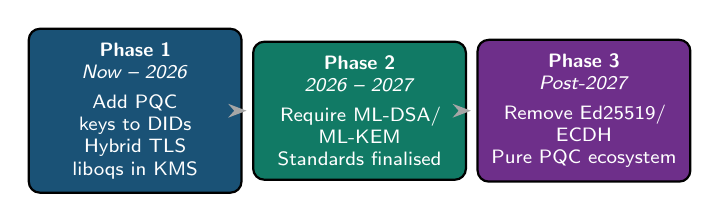
\begin{tikzpicture}[
  font=\sffamily\fontsize{6.8pt}{8pt}\selectfont,
  >=Stealth,
  box/.style={
    rectangle, rounded corners=4pt,
    minimum width=2.45cm, minimum height=1.55cm,
    text width=2.35cm, align=center,
    draw, thick, text=white, inner sep=5pt
  },
  arrow/.style={->, thick, gray!70, shorten >=2pt, shorten <=2pt}
]
  \node[box, fill=phase1] (p1) at (0,0)
    {\textbf{Phase 1}\\\textit{Now -- 2026}\\[3pt]
     Add PQC keys to DIDs\\Hybrid TLS\\liboqs in KMS};

  \node[box, fill=phase2] (p2) at (2.85,0)
    {\textbf{Phase 2}\\\textit{2026 -- 2027}\\[3pt]
     Require ML-DSA/\\ML-KEM\\Standards finalised};

  \node[box, fill=phase3] (p3) at (5.7,0)
    {\textbf{Phase 3}\\\textit{Post-2027}\\[3pt]
     Remove Ed25519/\\ECDH\\Pure PQC ecosystem};

  \draw[arrow] (p1.east) -- (p2.west);
  \draw[arrow] (p2.east) -- (p3.west);
\end{tikzpicture}
\caption{Phased PQC migration for DID ecosystems.
  Phase~1 is actionable today using NIST FIPS and community
  drafts~\cite{nist204,linkedin2024}.}
\label{fig:phases}
\end{figure}

%% ═══════════════════════════════════════════════════════════════════════════
\section{Modern IAM: Passwordless and JIT Access}
%% ═══════════════════════════════════════════════════════════════════════════

\subsection{Passwordless Authentication}

FIDO2/WebAuthn passkeys and biometric platform authenticators
eliminate the password as an attack surface.  Passkeys are ``nearly
immune to phishing'' and ``significantly improving user satisfaction
by removing password frustration''~\cite{ping2024pass}.  Microsoft
recommends passwordless as the default, with four options: Windows
Hello for Business, Microsoft Authenticator, FIDO2 passkeys, and
certificate-based authentication~\cite{msft2024}.

\subsection{JIT Access, CAE, and Policy Engines}

\emph{Just-in-Time (JIT) access} grants elevated roles for short
on-demand windows, eliminating standing privilege---the class of risk
exploited in the Change Healthcare breach.  \emph{Continuous Access
Evaluation (CAE)} revokes tokens mid-session on risk-condition changes
(device compliance drop, anomalous location) rather than at token
expiry, implementing ZTA's continuous-verification principle at the
session layer.  Policy engines (OPA/Rego, vendor-native rule sets)
evaluate attributes, risk scores, and contextual signals to make
fine-grained access decisions continuously, not only at authentication
time.

\subsection{Vendor Comparison Matrix}

Table~\ref{tab:vendors} compares eight leading IAM platforms across
deployment model, passwordless support, JIT/PAM capability, policy
engine, and indicative pricing.

%% ═══════════════════════════════════════════════════════════════════════════
%% TABLE 2 — IAM Vendor Comparison (two-column span)
%% ═══════════════════════════════════════════════════════════════════════════
\begin{table*}[t]
\caption{IAM vendor comparison matrix (2025). Pricing indicative.}
\label{tab:vendors}
\small
\setlength{\tabcolsep}{4.5pt}
\begin{tabularx}{\textwidth}{@{}
  p{1.7cm}          % Vendor
  p{1.6cm}          % Deploy
  p{2.8cm}          % Passwordless MFA
  p{2.4cm}          % JIT / PAM
  p{2.4cm}          % Policy Engine
  X                 % Base Pricing (fills remainder)
@{}}
\toprule
\textbf{Vendor} & \textbf{Deploy} & \textbf{Passwordless MFA} &
\textbf{JIT / PAM} & \textbf{Policy Engine} & \textbf{Base Pricing} \\
\midrule
Okta            & Cloud SaaS   & FIDO2, WebAuthn, OATH, push, email magic links~\cite{okta2024}
                               & Okta Privileged Access
                               & Adaptive MFA; workflow automation
                               & CIAM Enterprise $\approx$\$3k/mo \\
\addlinespace[3pt]
Microsoft Entra ID & Cloud     & Windows Hello, FIDO2, OATH, Authenticator~\cite{msft2024}
                               & Azure PIM; Identity Governance
                               & Conditional Access; CAE
                               & E5 $\approx$\$9/user/mo \\
\addlinespace[3pt]
Ping Identity   & SaaS/on-prem & FIDO2, biometrics, mobile push~\cite{ping2024pass}
                               & PingOne Privileged Access
                               & PingIntelligence risk scoring
                               & Enterprise (contact) \\
\addlinespace[3pt]
ForgeRock       & Cloud/on-prem & FIDO2, biometrics, SMS, email OTP
                               & ForgeRock Privileged Identity
                               & Policy trees; identity analytics
                               & $\approx$\$6--\$10/user/mo \\
\addlinespace[3pt]
CyberArk Idaptive & Cloud      & FIDO2, biometrics, SMS, OTP
                               & Built-in JIT + PAM workflows
                               & Adaptive policies; risk analytics
                               & Included in PAM plans \\
\addlinespace[3pt]
Auth0 (Okta CIAM) & SaaS       & FIDO2, WebAuthn, SMS, email OTP
                               & Not included
                               & Rules; extensible auth pipelines
                               & Free tier; Enterprise \$23k/yr+ \\
\addlinespace[3pt]
IBM Security Verify & Cloud/on-prem & FIDO2/WebAuthn, OATH, email OTP
                               & Worker token-based JIT
                               & Risk-based policies; analytics
                               & $\approx$\$3/user/mo \\
\addlinespace[3pt]
SailPoint       & Cloud        & SSO delegates MFA to IdP
                               & IdentityIQ access requests
                               & Governance policies; IoT
                               & Enterprise by quote \\
\bottomrule
\end{tabularx}
\end{table*}

%% ═══════════════════════════════════════════════════════════════════════════
\section{Compliance Drivers and Regulatory Mapping}
%% ═══════════════════════════════════════════════════════════════════════════

\subsection{Regulatory Landscape}

Table~\ref{tab:compliance} maps six regulatory frameworks to specific
ZTA controls.  The common pattern: authentication controls map to the
\emph{Identity} pillar; asset requirements to \emph{Device};
segmentation to \emph{Network}; logging to the \emph{Visibility}
pillar.

%% ═══════════════════════════════════════════════════════════════════════════
%% TABLE 3 — Regulatory Mapping (two-column span)
%% ═══════════════════════════════════════════════════════════════════════════
\begin{table*}[t]
\caption{Regulatory compliance drivers mapped to ZTA controls.}
\label{tab:compliance}
\small
\setlength{\tabcolsep}{5pt}
\begin{tabularx}{\textwidth}{@{}
  p{3.0cm}   % Regulation
  p{1.6cm}   % Deadline
  p{5.5cm}   % Key Requirements
  X          % ZTA Control Mapping
@{}}
\toprule
\textbf{Regulation} & \textbf{Deadline} &
\textbf{Key Requirements} & \textbf{ZTA Control Mapping} \\
\midrule
OMB M-22-09 + EO~14028~\cite{omb2022} & FY2024
  & Phishing-resistant MFA; remove password rotation; complete device inventory
  & Identity pillar (FIDO2/PIV); Device pillar (MDM); continuous monitoring \\
\addlinespace[3pt]
DoD ZT Strategy~\cite{dod2022} & FY2027
  & 50\% systems under continuous authorisation; MFA (PIV/CAC); microsegmentation
  & All CISA pillars; PEP per workload \\
\addlinespace[3pt]
NYDFS Part~500~\cite{nydfs2025} & Nov 2025
  & Universal MFA every user/system; dual CEO+CISO attestation; PAM+EDR (Class~A)
  & Identity (universal MFA); Device (EDR); Audit (dual sign-off) \\
\addlinespace[3pt]
DORA & 2025
  & Cyber resilience testing; identity \& access; ICT third-party risk
  & ZT segmentation; vendor access gating; continuous posture assessment \\
\addlinespace[3pt]
NIST SP~800-207 / SP~1800-35~\cite{nist800207} & Reference
  & ZTA logical architecture (PE/PA/PEP); five pillars; CDM
  & End-to-end reference; maps to NIST~800-53 Rev~5 \\
\addlinespace[3pt]
PCI-DSS v4.0 / HIPAA / GDPR & Sector-specific
  & Risk-based auth; unique user IDs + logging; privacy by design
  & Access enforcement; audit logs; data minimisation \\
\bottomrule
\end{tabularx}
\end{table*}

\subsection{NYDFS Part 500: Statutory Urgency}

NYDFS Part~500 is the most prescriptive US financial ZTA mandate.
\textbf{November~1, 2025} is the final deadline for universal
MFA---every user, every system, every time---with no exceptions.  The
2023 Second Amendment introduced personal liability: both CEO and CISO
must sign compliance attestations with evidence-based documentation;
NYDFS has levied fines up to \$30M for non-compliance~\cite{nydfs2025}.

%% ═══════════════════════════════════════════════════════════════════════════
\section{Platform Consolidation and Cloud-Native ZTA}
%% ═══════════════════════════════════════════════════════════════════════════

Enterprises are consolidating from dozens of point products into unified
identity-centric ZTA platforms.  A representative architecture contains
three tiers: (1)~\emph{Identity + Directory}: cloud IdP plus enterprise
directory sync; (2)~\emph{Context + Policy}: PDP ingesting device
posture, user behaviour, and threat intelligence; and
(3)~\emph{Enforcement}: distributed PEPs---ZTNA gateways, CASB proxies,
service mesh sidecars, and API gateways---implementing PDP decisions.

Figure~\ref{fig:zta-arch} illustrates the authentication flow.
Migration typically proceeds in three waves: identity and SSO
migration; network edge replacement (ZTNA replacing VPN, cloud
workload microsegmentation); and legacy VPN/firewall decommission.

%%
%% FIGURE 2 — ZTA Logical Architecture (single column)
%%
\begin{figure}[h]
\centering
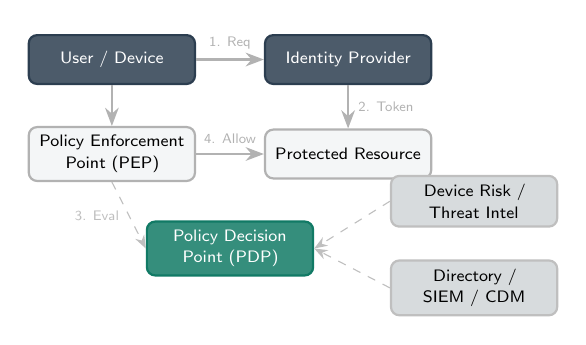
\begin{tikzpicture}[
  font=\sffamily\fontsize{6.5pt}{7.8pt}\selectfont,
  >=Stealth,
  entity/.style={
    rectangle, rounded corners=3pt,
    minimum width=2.0cm, minimum height=0.62cm,
    text width=1.9cm, align=center,
    draw=gray!60, thick, fill=lightbg, inner sep=3pt
  },
  core/.style={
    entity, fill=idcol!85, text=white, draw=idcol
  },
  pdp/.style={
    entity, fill=phase2!85, text=white, draw=phase2
  },
  ctx/.style={
    entity, fill=midgray!60, draw=gray!50
  },
  arr/.style={->, thick, gray!60},
  darr/.style={->, dashed, gray!50}
]

  %% Nodes
  \node[core]  (user)   at (0.0, 2.4)  {User / Device};
  \node[core]  (idp)    at (3.0, 2.4)  {Identity Provider};
  \node[entity](pep)    at (0.0, 1.2)  {Policy Enforcement\\Point (PEP)};
  \node[entity](res)    at (3.0, 1.2)  {Protected Resource};
  \node[pdp]   (pdp)    at (1.5, 0.0)  {Policy Decision\\Point (PDP)};
  \node[ctx]   (ctx)    at (4.6, 0.6)  {Device Risk /\\Threat Intel};
  \node[ctx]   (dir)    at (4.6,-0.5)  {Directory /\\SIEM / CDM};

  %% Data-plane (solid)
  \draw[arr] (user.east)  -- node[above, font=\fontsize{5.5pt}{6pt}\sffamily]{1. Req}   (idp.west);
  \draw[arr] (idp.south)  -- node[right, font=\fontsize{5.5pt}{6pt}\sffamily]{2. Token} (res.north);
  \draw[arr] (pep.east)   -- node[above, font=\fontsize{5.5pt}{6pt}\sffamily]{4. Allow} (res.west);
  \draw[arr] (user.south) -- (pep.north);

  %% Control-plane (dashed)
  \draw[darr] (pep.south)  -- node[left,  font=\fontsize{5.5pt}{6pt}\sffamily]{3. Eval} (pdp.west);
  \draw[darr] (ctx.west)   -- (pdp.east);
  \draw[darr] (dir.west)   -- (pdp.east);

\end{tikzpicture}
\caption{Unified ZTA logical architecture.  Solid arrows: data-plane
  request/token/allow flow.  Dashed arrows: control-plane policy query
  and telemetry feed.}
\label{fig:zta-arch}
\end{figure}

%% ═══════════════════════════════════════════════════════════════════════════
\section{Attacker Adaptation to ZTA}
%% ═══════════════════════════════════════════════════════════════════════════

As ZTA matures, attackers shift to allowed vectors.  Table~\ref{tab:ttps}
catalogues five evolved threat profiles.  Research notes that a mature
ZTA still only blocks approximately half of attacks~\cite{darkreading2024};
Google (BeyondCorp) and Microsoft have published that continuous trust
evaluation---not static session authentication---is the decisive
differentiator~\cite{msft2024}.

Figure~\ref{fig:ttp-map} maps each TTP to the ZTA layer it targets.

%% ═══════════════════════════════════════════════════════════════════════════
%% TABLE 4 — Evolved TTPs (two-column span)
%% ═══════════════════════════════════════════════════════════════════════════
\begin{table*}[t]
\caption{Evolved attacker TTPs against mature ZTA, with mitigations.}
\label{tab:ttps}
\small
\setlength{\tabcolsep}{5pt}
\begin{tabularx}{\textwidth}{@{}
  p{3.2cm}   % TTP
  p{5.0cm}   % Mechanism
  X          % Mitigation
@{}}
\toprule
\textbf{TTP} & \textbf{Mechanism} & \textbf{Mitigation} \\
\midrule
Token / credential theft
  & Pass-the-cookie; OAuth token memory exfil; MFA push fatigue
  & CAE revocation; short-lived tokens; UEBA anomaly scoring on token usage \\
\addlinespace[3pt]
IdP supply-chain compromise
  & Attack identity providers directly (cf.\ SolarWinds, Okta~2022)
  & Redundant multi-cloud IdP; out-of-band admin action verification \\
\addlinespace[3pt]
Device posture spoofing
  & Jailbreak device to appear compliant; spoof TPM attestation
  & Hardware-bound FIDO2/TPM attestation; multi-source posture fusion \\
\addlinespace[3pt]
Lateral movement within permitted segments
  & Compromise an authorised service, pivot to adjacent permitted resources
  & Strict per-service least-privilege scoping; continuous east-west monitoring \\
\addlinespace[3pt]
Insider threat / social engineering
  & Valid credentials on authorised device used for exfiltration
  & JIT with session recording; UEBA baseline deviation alerts; DLP on authorised transfers \\
\bottomrule
\end{tabularx}
\end{table*}

%%
%% FIGURE 3 — Attacker TTP targeting map (single column)
%%
\begin{figure}[h]
\centering
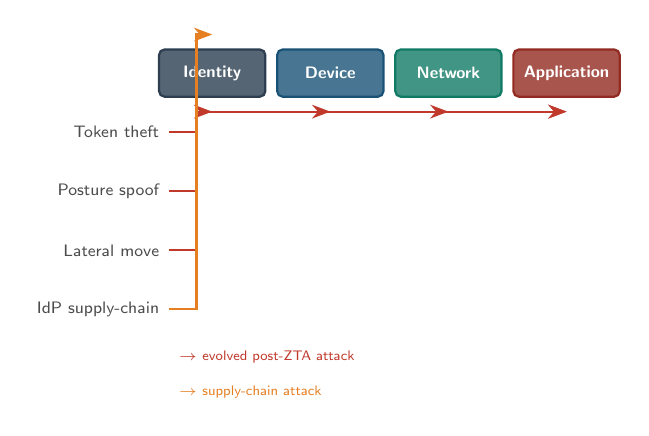
\begin{tikzpicture}[
  font=\sffamily\fontsize{6.5pt}{7.8pt}\selectfont,
  >=Stealth
]
  %% ── ZTA Layer header row ──────────────────────────────────────────────
  \def\layerw{1.35cm}
  \def\layerh{0.6cm}
  \def\gap{1.5cm}

  %% Pillar boxes at y=0
  \foreach \lbl/\col/\xi in {
    Identity/idcol/0,
    Device/devcol/1,
    Network/netcol/2,
    Application/appcol/3}
  {
    \node[rectangle, rounded corners=2pt,
          minimum width=\layerw, minimum height=\layerh,
          fill=\col!80, text=white, draw=\col, thick,
          align=center, inner sep=2pt,
          font=\sffamily\fontsize{6pt}{7pt}\selectfont\bfseries]
      (layer-\xi) at (\xi*\gap, 0) {\lbl};
  }

  %% TTP labels on left
  \foreach \lbl/\yi in {
    {Token theft}/1,
    {Posture spoof}/2,
    {Lateral move}/3,
    {IdP supply-chain}/4}
  {
    \node[anchor=east,
          font=\sffamily\fontsize{6pt}{7pt}\selectfont,
          text=black!70]
      (ttp-\yi) at (-0.55, -\yi*0.75) {\lbl};
  }

  %% Attack arrows: which pillars does each TTP target?
  % Token theft -> Identity, Application
  \draw[->, thick, attackred]
    (ttp-1.east) -- ++(0.35,0) |- ([yshift=-5pt]layer-0.south);
  \draw[->, thick, attackred]
    (ttp-1.east) -- ++(0.35,0) |- ([yshift=-5pt]layer-3.south);

  % Posture spoof -> Device
  \draw[->, thick, attackred]
    (ttp-2.east) -- ++(0.35,0) |- ([yshift=-5pt]layer-1.south);

  % Lateral move -> Network, Application
  \draw[->, thick, attackred]
    (ttp-3.east) -- ++(0.35,0) |- ([yshift=-5pt]layer-2.south);
  \draw[->, thick, attackred]
    (ttp-3.east) -- ++(0.35,0) |- ([yshift=-5pt]layer-3.south);

  % IdP supply-chain -> Identity (orange, from above)
  \draw[->, thick, supplyorg]
    (ttp-4.east) -- ++(0.35,0) |- ([yshift=5pt]layer-0.north);

  %% Legend
  \node[anchor=west, font=\fontsize{5.5pt}{6.5pt}\sffamily, text=attackred]
    at (-0.55, -3.6) {$\rightarrow$ evolved post-ZTA attack};
  \node[anchor=west, font=\fontsize{5.5pt}{6.5pt}\sffamily, text=supplyorg]
    at (-0.55, -4.05) {$\rightarrow$ supply-chain attack};

\end{tikzpicture}
\caption{Attacker TTP targeting map against ZTA layers.  Red arrows:
  evolved post-ZTA attacks.  Orange arrow: supply-chain attack targeting
  the identity layer.}
\label{fig:ttp-map}
\end{figure}

%% ═══════════════════════════════════════════════════════════════════════════
\section{User Experience and Usability}
%% ═══════════════════════════════════════════════════════════════════════════

\subsection{Friction Reduction}

Passwordless methods eliminate password frustration while strengthening
security~\cite{ping2024pass}.  Adaptive MFA applies challenges only when
risk is elevated; routine low-risk sessions proceed via SSO with silent
background posture checks.  Five actionable UX principles:

\begin{description}[leftmargin=1.4em, labelindent=0pt,
                    topsep=2pt, itemsep=1pt, labelsep=0.5em]
  \item[UX1.] Passwordless by default (FIDO2/WebAuthn + biometric fallback).
  \item[UX2.] Adaptive step-up only on anomaly (new device, unusual location,
              sensitive resource, or elevated risk score).
  \item[UX3.] Consistent branded portal across all applications.
  \item[UX4.] Self-service authenticator enrollment (reduces help-desk volume).
  \item[UX5.] Graceful fallback that never degrades to password-only.
\end{description}

\subsection{UX Metrics}

Key operational metrics: login success rate ($>$98\%); mean time to
authenticate (seconds vs.\ legacy VPN baseline); help-desk auth
tickets per 100 users/month (target $\leq$3); MFA challenge rate per
session (target ${<}$20\%); quarterly user satisfaction score
(directionally improving).  A/B testing of MFA methods under identical
risk conditions reveals completion rates and abandonment patterns that
inform policy calibration.

%% ═══════════════════════════════════════════════════════════════════════════
\section{ZTA Resilience and Graceful Degradation}
%% ═══════════════════════════════════════════════════════════════════════════

\subsection{Identity as Critical Infrastructure}

Identity and policy systems are critical infrastructure: if the IdP
or PDP becomes unreachable, users may be completely locked
out~\cite{hackernews2024}.  Cloud identity outages can render
authentication flows unusable even when the identity service itself
is running---dependencies like DNS, shared databases, and upstream
services fail the broader flow~\cite{hackernews2024}.  Identity outages
``should trigger the highest level of incident
response''~\cite{hackernews2024}.

\subsection{Failure Mode Taxonomy}

Table~\ref{tab:failures} classifies six ZTA failure modes with
resilience architecture responses.

%% ═══════════════════════════════════════════════════════════════════════════
%% TABLE 5 — Failure Modes (two-column span)
%% ═══════════════════════════════════════════════════════════════════════════
\begin{table*}[t]
\caption{ZTA failure modes and resilience architecture mitigations.}
\label{tab:failures}
\small
\setlength{\tabcolsep}{5pt}
\begin{tabularx}{\textwidth}{@{}
  p{3.5cm}   % Failure Mode
  p{4.5cm}   % Impact
  X          % Mitigation
@{}}
\toprule
\textbf{Failure Mode} & \textbf{Impact} & \textbf{Mitigation} \\
\midrule
IdP regional outage
  & Complete lockout for affected region
  & Multi-region active/active; cross-cloud IdP~\cite{hackernews2024} \\
\addlinespace[3pt]
DNS failure
  & Auth flows break despite healthy IdP
  & Multiple resolvers; local DNS cache \\
\addlinespace[3pt]
PDP policy engine down
  & PEPs cannot evaluate access requests
  & Cached decisions (time-limited TTL); pre-computed group memberships \\
\addlinespace[3pt]
Shared cloud dependency failure
  & Auth breaks across all dependent services simultaneously
  & Distinct cloud providers for IdP and CDN; circuit breakers~\cite{hackernews2024} \\
\addlinespace[3pt]
Endpoint unreachable
  & Device attestation unverifiable
  & Cached posture (short TTL); hardware TPM \\
\addlinespace[3pt]
Full network isolation (OT/offline)
  & Central IdP unreachable
  & FIDO2 device-bound passkeys; offline cached policies (reduced privilege) \\
\bottomrule
\end{tabularx}
\end{table*}

\subsection{Resilience Design Principles}

``Identity systems must be engineered to fail gracefully. When
infrastructure outages are inevitable, access control should degrade
predictably, not completely collapse''~\cite{hackernews2024}.  Five
design principles guide this engineering:

\textbf{Multi-cloud/hybrid fallback.}  Separate cloud providers for
IdP and its DNS dependencies; maintain an on-premises or
alternative-cloud emergency IdP.

\textbf{Credential and decision caching.}  Devices carry time-limited
cached validity assertions and pre-computed policy decisions.  ``Allowing
limited access, based on cached attributes \ldots{} can dramatically
reduce operational and reputational damage''~\cite{hackernews2024}.

\textbf{Graceful degradation modes.}  Define explicitly what access is
permitted during outages: basic read-only access to critical resources;
VPN-like fallback with stricter logging.  Document and test quarterly.

\textbf{Failover SLA requirements.}  Negotiate and verify multi-region,
multi-provider SLAs.  Understand shared risk domains: co-hosted IdP
and directory may fail together.

\textbf{Endpoint autonomy.}  For isolated environments, devices carry
hardware-bound cryptographic credentials (FIDO2 passkeys, PIV smart
cards) and cached policies for minimal operation.

Figure~\ref{fig:resilience} illustrates the reference resilience
architecture.

%%
%% FIGURE 4 — Resilience Architecture (single column)
%%
\begin{figure}[h]
\centering
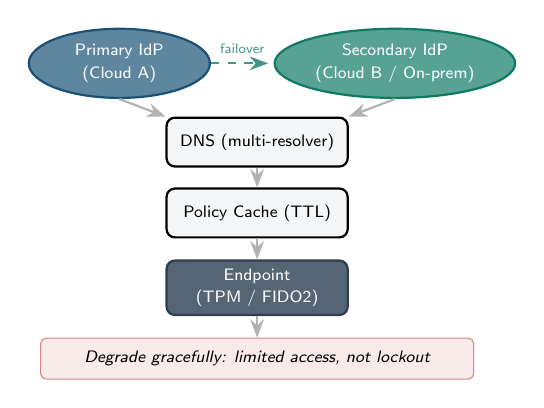
\begin{tikzpicture}[
  font=\sffamily\fontsize{6.5pt}{8pt}\selectfont,
  >=Stealth,
  cloud/.style={
    ellipse, draw, thick,
    minimum width=2.3cm, minimum height=0.7cm,
    align=center, inner sep=2pt
  },
  rect/.style={
    rectangle, rounded corners=3pt, draw, thick,
    minimum width=2.3cm, minimum height=0.62cm,
    align=center, inner sep=3pt
  },
  arr/.style={->, thick, gray!60},
  farr/.style={->, dashed, thick, phase2!80, shorten >=2pt}
]
  %% Primary IdP
  \node[cloud, fill=phase1!70, text=white, draw=phase1]
    (idp1) at (0, 2.0) {Primary IdP\\(Cloud A)};

  %% Secondary IdP
  \node[cloud, fill=phase2!70, text=white, draw=phase2]
    (idp2) at (3.5, 2.0) {Secondary IdP\\(Cloud B / On-prem)};

  %% DNS
  \node[rect, fill=lightbg] (dns) at (1.75, 1.0) {DNS (multi-resolver)};

  %% Policy cache
  \node[rect, fill=lightbg] (cache) at (1.75, 0.1) {Policy Cache (TTL)};

  %% Endpoint
  \node[rect, fill=idcol!80, text=white, draw=idcol]
    (ep) at (1.75, -0.85) {Endpoint\\(TPM / FIDO2)};

  %% Degradation banner
  \node[rectangle, rounded corners=2pt,
        draw=attackred!60, fill=attackred!10,
        minimum width=5.5cm, minimum height=0.52cm,
        align=center, font=\fontsize{6pt}{7pt}\sffamily\itshape,
        inner sep=3pt]
    (banner) at (1.75, -1.75)
    {Degrade gracefully: limited access, not lockout};

  %% Connections
  \draw[arr]  (idp1.south)  -- (dns.north west);
  \draw[arr]  (idp2.south)  -- (dns.north east);
  \draw[arr]  (dns.south)   -- (cache.north);
  \draw[arr]  (cache.south) -- (ep.north);
  \draw[farr] (idp1.east)   -- node[above,
    font=\fontsize{5.5pt}{6pt}\sffamily]{failover} (idp2.west);
  \draw[arr]  (ep.south)    -- (banner.north);

\end{tikzpicture}
\caption{ZTA resilience reference architecture: active/active cross-cloud
  IdPs; multi-resolver DNS; endpoint policy cache.  Failover is automatic;
  degradation provides reduced-privilege access rather than complete
  lockout~\cite{hackernews2024}.}
\label{fig:resilience}
\end{figure}

%% ═══════════════════════════════════════════════════════════════════════════
\section{Discussion}
%% ═══════════════════════════════════════════════════════════════════════════

\subsection{PQC Migration Urgency vs.\ Standard Readiness}

The tension between ``harvest now, decrypt later'' urgency and the
absence of finalised PQC-DID standards is the defining challenge of
Phase~1.  Community consensus---and NIST's explicit recommendation to
begin adoption now~\cite{nist204}---supports hybrid deployment (adding
PQC keys alongside classical keys) as safe and immediately actionable.
Waiting for formal W3C PQC-DID standardisation ($\approx$2027) creates
unacceptable exposure for organisations handling long-lived sensitive
identities.

\subsection{Implicit Trust Creep as a ZTA Failure Mode}

A consistent pattern across ZTA deployments is that
\emph{implicit trust creep}---gradual re-accumulation of standing
privileges, assumed-compliant devices, and trusted services without
continuous verification---is the primary mechanism through which ZTA
posture degrades after initial deployment.  JIT access, CAE, and
scheduled policy re-certification are the operational mechanisms that
prevent this degradation.

\subsection{Resilience as First-Class Requirement}

Identity outages convert ZTA's security strength into a
business con\-ti\-nu\-ity liability.  The solution is \emph{resilient ZTA}:
multi-cloud redundancy, credential caching, and explicitly designed
graceful-degradation modes.  This must be designed in from the start,
not retrofitted.

\subsection{Limitations}

Vendor pricing data are indicative and change frequently.
Listing~\ref{lst:did} is a conceptual skeleton; production
implementation requires validated multicodec registrations and
\texttt{liboqs} library support.  ML-DSA key/signature sizes in
Table~\ref{tab:pqc-alg} are for NIST Level~3; Level~2 and Level~5
variants have different parameters.

%% ═══════════════════════════════════════════════════════════════════════════
\section{Conclusion}
%% ═══════════════════════════════════════════════════════════════════════════

This paper provided a comprehensive treatment of the intersection of PQC,
decentralised identity, modern IAM, regulatory compliance, attacker
adaptation, UX, and ZTA resilience.

NIST's 2024 finalisation of FIPS~203/204/205 makes hybrid PQC migration
actionable today.  The recommended posture is a Hybrid DID Document with
both Ed25519 and ML-DSA verification methods, Hybrid TLS
(X25519~+~ML-KEM), and JOSE-PQC for DIDComm, with a three-phase
migration roadmap to pure-PQC by post-2027~\cite{nist204,linkedin2024}.

Modern IAM has decisively shifted to passwordless authentication via
FIDO2/WebAuthn credentials, JIT privilege, and CAE---available across
all eight surveyed vendors.  Regulatory mandates (OMB~M-22-09,
NYDFS~Part~500, DORA) convert ZTA from best practice to legal
obligation.

As ZTA matures, attackers adapt: token theft, IdP supply-chain
compromise, posture spoofing, and lateral movement within permitted
segments define the post-ZTA threat surface.  Hardware-bound attestation,
continuous behavioural analytics, and strict least-privilege scoping are
the necessary responses.

Finally, identity systems are critical infrastructure whose failure modes
must be explicitly designed against.  Multi-cloud redundancy, policy
caching, and graceful degradation that provides minimal access rather than
complete lockout~\cite{hackernews2024} are not optional
enhancements---they are architectural requirements.

%% ─── References ────────────────────────────────────────────────────────────
\sloppy
\bibliographystyle{ACM-Reference-Format}
\begin{thebibliography}{13}

\bibitem{nist204}
NIST.
\newblock {FIPS 204: Module-Lattice-Based Digital Signature Standard}.
\newblock August 2024.
\newblock \url{https://csrc.nist.gov/pubs/fips/204/final}

\bibitem{linkedin2024}
LinkedIn.
\newblock Future-proofing decentralized identity: Integrating {PQC} into
  {Hyperledger Indy \& DID:WEB}.
\newblock 2024.
\newblock \url{https://www.linkedin.com/}

\bibitem{ping2024federal}
Ping Identity.
\newblock Addressing the quantum threat in the {US} federal government.
\newblock 2024.
\newblock \url{https://www.pingidentity.com/}

\bibitem{frontiers2024}
Frontiers.
\newblock Complying with the {NIST PQC} standards and decentralizing {AI}:
  Methodology for quantum-resistant digital identity.
\newblock 2024.
\newblock \url{https://www.frontiersin.org/}

\bibitem{ping2024pass}
Ping Identity.
\newblock Discover secure \& convenient passwordless authentication.
\newblock 2024.
\newblock \url{https://www.pingidentity.com/}

\bibitem{msft2024}
Microsoft.
\newblock {Microsoft Cloud Security Benchmark v2: Identity Management}.
\newblock Microsoft Learn, 2024.
\newblock \url{https://learn.microsoft.com/}

\bibitem{okta2024}
Okta.
\newblock Plans and pricing.
\newblock 2024.
\newblock \url{https://www.okta.com/pricing/}

\bibitem{omb2022}
White House / OMB\@.
\newblock {M-22-09: Moving the U.S. Government Toward Zero Trust Cybersecurity
  Principles}.
\newblock January 2022.
\newblock \url{https://www.whitehouse.gov/}

\bibitem{dod2022}
Carahsoft.
\newblock {DoD} Zero Trust Strategy Release.
\newblock 2022.
\newblock \url{https://www.carahsoft.com/}

\bibitem{nydfs2025}
Beyond Identity.
\newblock {NYDFS Part 500} in 2025: Key deadlines, new requirements, and
  compliance strategies.
\newblock 2025.
\newblock \url{https://www.beyondidentity.com/}

\bibitem{nist800207}
{NIST NCCoE}.
\newblock {NIST Guidance on Implementing a ZTA (SP 1800-35)}.
\newblock December 2024.
\newblock \url{https://csrc.nist.gov/}

\bibitem{darkreading2024}
Dark Reading / Gartner.
\newblock Companies struggle with zero trust as attackers adapt to get around
  it.
\newblock 2024.
\newblock \url{https://www.darkreading.com/}

\bibitem{hackernews2024}
The Hacker News.
\newblock When cloud outages ripple across the internet.
\newblock 2024.
\newblock \url{https://thehackernews.com/}

\end{thebibliography}

\end{document}
